\section{\textbf{Our Approach}}\label{sec:main}
 \subsection{ Possible Solutions - Video Streaming Mixer Library
}


Parse HLS manifest into object representations
Implement algorithm to identify matching video streams

 \begin{itemize}

     \item Strategy 1: set Filter against first element’s attributes
     \item  Strategy 2: set intersection for matching attributes

 \end{itemize}
 The output should be a master HLS manifest of a playlist including all matching video streams

 
\begin{figure}

\centering
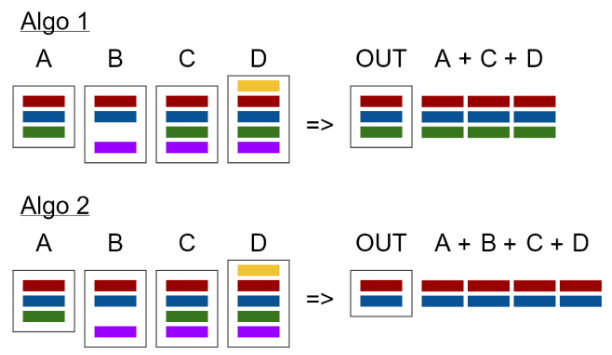
\includegraphics[scale=0.50]{figures/PossibleSolutions.png}
\caption{Possible Solutions }
\label{fig:IMT_2020_Use-cases}
\end{figure}


 
 For strategy 1, we have three variant playlists and the output also contains only three playlists. But these playlists are now longer, because they concatenate the matching playlists into a single red, a single blue and a single green playlists with all the segments from inputs A, B, C and D. While playlists purple and yellow use e.g. a different resolution and are not present in the first input A and thus are not used. 
For strategy 2, we see that only the intersection of variant playlists from all inputs is used. Two variants with the same resolution have been identified across all inputs, red and blue, so only two variant playlists should be in the output manifest. Each one will include all concatenated segments from all inputs matching the respective representation.
Finally, handling the playlists that have been identified as belonging to the same representation (resolution, bitrate). Realize that the output manifest, that needs to be written, can never have more media playlists than any of the input sources by itself. Do not add more media playlists to the master manifest. Instead, given the found media playlists using the same representation, concatenate these into a single media playlist and only that new playlist should be part of the master manifest output.




\begin{figure}

\centering
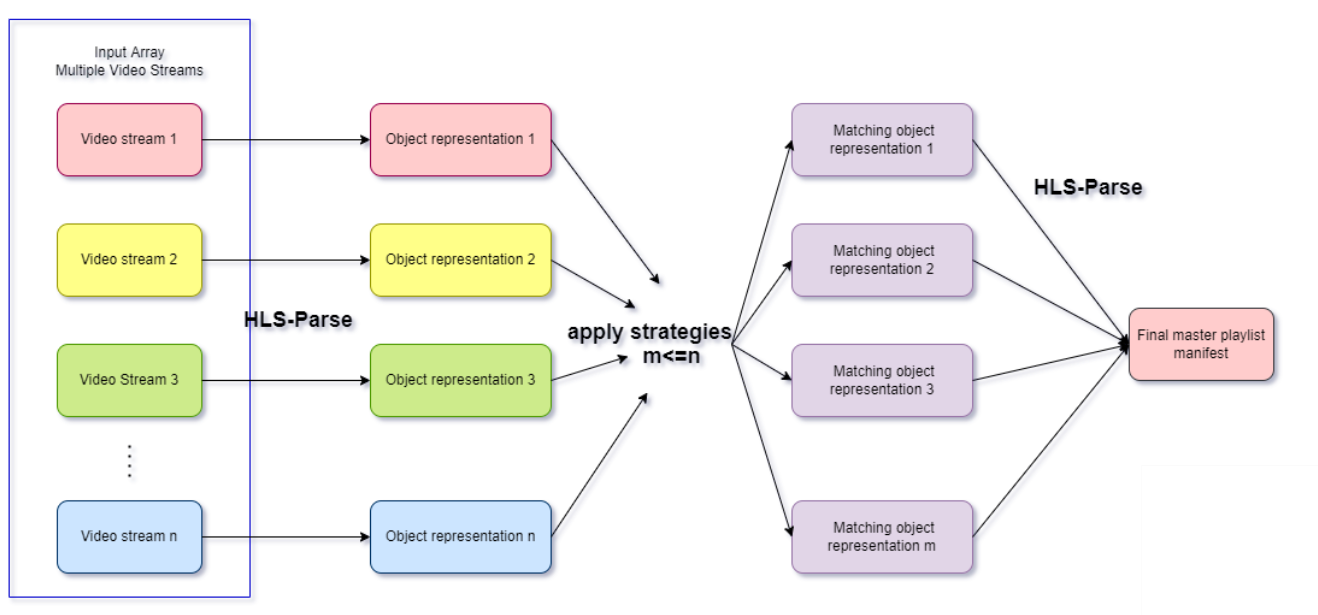
\includegraphics[scale=0.32]{figures/PossibleSolutions2.png}
\caption{Possible Solutions 2 }
\label{fig:IMT_2020_Use-cases}
\end{figure}





************************
here only to be familiar with the latex Symbols 

{\BibTeX} does not work by magic. It doesn't get the bibliographic
data from thin air but from .bib files. If you use {\BibTeX} to produce a
bibliography you must send the .bib files. 

{\LaTeX} can't read your mind. If you assign the same label to a
subsubsection and a table, you might find that Table I has been cross
referenced as Table IV-B3. 

{\LaTeX} does not have precognitive abilities. If you put a
\verb|\label| command before the command that updates the counter it's
supposed to be using, the label will pick up the last counter to be
cross referenced instead. In particular, a \verb|\label| command
should not go before the caption of a figure or a table.

Do not use \verb|\nonumber| inside the \verb|{array}| environment. It
will not stop equation numbers inside \verb|{array}| (there won't be
any anyway) and it might stop a wanted equation number in the
surrounding equation.